%%%%%%%%%%%%%%%%%%%%%%%%%%%%%%%%%%%%%%%%%%%%%%%%%%%%%%%%%%%%%%%%%%%%%%%%
%                                                                      %
%     File: Thesis_Implementation.tex                                  %
%     Tex Master: Thesis.tex                                           %
%                                                                      %
%     Author: Andre C. Marta                                           %
%     Last modified :  2 Jul 2015                                      %
%                                                                      %
%%%%%%%%%%%%%%%%%%%%%%%%%%%%%%%%%%%%%%%%%%%%%%%%%%%%%%%%%%%%%%%%%%%%%%%%

\chapter{Implementation}
\label{chapter:implementation}

This section will go in depth on the implementation of the concepts presented in the chapter \ref{chapter:background}. The plane model to be controlled was firstly implemented and verified. The first goal after this first step was to design a controller that would allow the aircraft to follow a trajectory from several position waypoints through time. The influence of certain parameters and knowledge of the exact plane model will be studied and discussed in chapter \ref{chapter:results}. The final goal will be to improve the controller and its robustness by reducing tracking error through the use of an adaptive neural network.

%%%%%%%%%%%%%%%%%%%%%%%%%%%%%%%%%%%%%%%%%%%%%%%%%%%%%%%%%%%%%%%%%%%%%%%%
\section{Plane Model}
\label{section:model}

The chosen commercial aircraft that will be simulated is the Boeing 737-200, an aircraft with over 30 years of service for which some information of flight parameters is readily available, such as weight, wing span and mean chord. The simulation was made in a cruise flight environment, at $200$ m/s velocity at $10000$ m above the ground. The chosen inertial matrix for this aircraft is given by
\begin{equation}
\begin{bmatrix}
1278369.56 & 0 & -135588.17\\
0 & 3781267.79 & 0\\
-135588.17 & 0 & 4877649.98
\end{bmatrix}
kg.m^2
\end{equation}
The ISA atmospheric model was used to measure the air density at any given height.
\begin{table}[htbp]
  \centering
  \caption{Boeing 737-2 parameters}
    \begin{tabular}{rr}
    \toprule
    Weight $m$ & $52390$ kg \\
    Wing Span $b$ & $28.35$ m \\
    Wing Area $S$ & $102.0$ m$^{2}$ \\
    Wing mean chord $\bar{c}$ & $4.35$ m \\
    Length $l$ & $30.53$ m \\
    \bottomrule
    \end{tabular}%
  \label{tab:b737_parameters}
\end{table}%
The time constants used for the actuators was $\xi_{\delta_i}50$ms and $\xi_T=4$s for the engines.
\subsection{Plane Dynamics}
\label{section:model/plane_dynamics}

In order to simulate the aircraft's fast dynamics, its moments must firstly be computed in order to use equation \ref{eq:fast_dynamics}. The torque caused by the actuators as modelled as equation \ref{eq:cdelta}, using
\begin{gather*}
C_{L_{\delta_{ail}}}=0.02 \quad rad^{-1}\\
C_{L_{\delta_{rud}}}=0.002 \quad rad^{-1}\\
C_{M_{\delta_{ele}}}=-0.003 \quad rad^{-1}\\
C_{N_{\delta_{ail}}}= -0.002 \quad rad^{-1}\\
C_{N_{\delta_{rud}}}= -0.07 \quad rad^{-1}
\end{gather*}
The remaining aerodynamic coefficients from equation \ref{eq:cmoment} were obtained from the work of Hector Escamilla Nuñez in \cite{hector}. In this work, neural networks were used to interpolate data from the USAF Stability and Control Digital Data Compendium. A two layer feed forward network, with a hidden sigmoid activation function and a linear output activation function, was then trained using the gathered data with the Bayesian Regulation training algorithm \cite{hector}. Indeed as stated previously, neural networks can approximate any continuous function according to the Universal Approximation Theorem. This method is therefore optimal to accurately approximate the variation of these coefficients that mainly vary with the angle of attack $\alpha$ and airspeed $V_a$. The only exception to this method was the drag coefficient, given for this aircraft by
\begin{equation}
C_D=0.0176+0.0515 C_L^2
\label{eq:cd_cl}
\end{equation}

The sum of the moments can be computed and used to obtain the rotation rates $p$, $q$ and $r$. Equation \ref{eq:euler2omega} can also be used and integrated to obtain the Euler angles. These will also be necessary for frame of reference changes, namely from body to earth and vice-versa. The aerodynamic forces were computed from equation \ref{eq:forces} using the outputs of the neural networks. The body forces and acceleration relative to the earth frame were then obtain from equations \ref{eq:body_forces} and \ref{eq:boddy_acc}. 
The effects of the wind were also taken into account by adding the wind speed to the integration of the acceleration of the aircraft relative to the earth as per \ref{eq:windtriangle}. At this point the values of $\alpha$ and $\beta$ were also obtained for their respective equations \ref{eq:alpha} and \ref{eq:beta}. 

A simplified block diagram of the plane simulator is given by figure \ref{fig:plane_model}.
\begin{figure}[!htb]
  \centering
  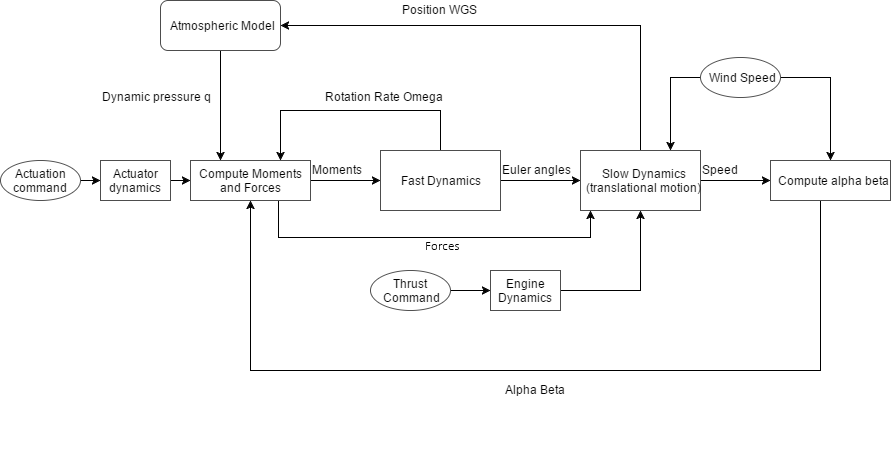
\includegraphics[width=0.75\textwidth]{Figures/PlaneModel.png}
  \caption[Plane dynamics simulator diagram]{Plane dynamics simulator diagram}
  \label{fig:plane_model}
\end{figure}
 

\section{Controller Implementation}
\label{section:control_implement}

To invert such a complex system, two layers of inversion are proposed by H. Escamilla \cite{hector}, namely for the fast and slow dynamics. Directly controlling these are three of the four actuator control inputs, the control surfaces for the aileron, elevon and rudder. These will therefore be the output of the nonlinear inversion control. To invert the fast dynamics the equation \ref{eq:fast_dynamics} must be differentiated once, to account for both the actuator dynamics \ref{eq:actuator_dynamics} and the effects of the wind. Doing so yields the jerk vector given by, as per \cite{hector}

\begin{equation}
\begin{bmatrix}
\ddot{p}\\
\ddot{q}\\
\ddot{r}
\end{bmatrix}
= \dfrac{1}{2}\rho SI^{-1} \left\lbrace V_a^2 C_\delta \xi
\begin{bmatrix}
\delta^d_{ail}-\delta_{ail}\\
\delta^d_{ele}-\delta_{ele}\\
\delta^d_{rud}-\delta_{rud}
\end{bmatrix}
+V_a^2C_c\dot{R_a}+2V_a\dot{V_a}\left(
\begin{bmatrix}
bC_l\\
\bar{c}C_m\\
bC_n
\end{bmatrix}
+ C_\delta 
\begin{bmatrix}
\delta_{ail}\\
\delta_{ele}\\
\delta_{rud}
\end{bmatrix}
\right) \right \rbrace + I^{-1}\left(\dfrac{1}{4}\rho SV_aC_k-I_n\right)\dot{\Omega}
\label{eq:jerk}
\end{equation}

Where

\begin{gather*}
I=
\begin{bmatrix}
A & 0 & -E\\
0 & B & 0\\
-E & 0 & C
\end{bmatrix}\\
I_n=
\begin{bmatrix}
-Eq & (C-B)r-Ep & (C-B)q\\
(A-C)r+2Ep & 0 & (A-C)p-2Er\\
(B-A)q & (B-A)p+Er & Eq
\end{bmatrix}\\
\xi=
\begin{bmatrix}
\dfrac{1}{\xi_{ail}} & 0 & 0\\
0 & \dfrac{1}{\xi_{ele}} & 0\\
0 & 0 & \dfrac{1}{\xi_{rud}}
\end{bmatrix}\\
C_c=
\begin{bmatrix}
0 & bC_{l_\beta} & -\dfrac{b^2}{2V_a^2}(C_{l_p}p+C_{l_r}r)\\
\bar{c}C_{m_\alpha} & 0 & -\dfrac{\bar{c}^2}{2V_a^2}C_{m_q}q\\
0 & bC_{n_\beta} & -\dfrac{b^2}{2V_a^2}(C_{n_p}p+C_{n_r}r)
\end{bmatrix}\\
C_k=
\begin{bmatrix}
b^2C_{l_p} & 0 & b^2C_{l_r}\\
0 & \bar{c}^2C_{m_q} & 0\\
b^2C_{n_p} & 0 & b^2C_{n_r}
\end{bmatrix}\\
\dot{Ra} =  [\dot{\alpha} \quad \dot{\beta} \quad \dot{V_a}]^T
\end{gather*}

To do a feedback linearisation, a pseudo input must be chosen, in this case $\tau = \ddot{\Omega}$. The feedback control law will therefore be, solving equation \ref{eq:jerk} to $\delta^d$,

\begin{equation}
\begin{bmatrix}
\delta^d_{ail}\\
\delta^d_{ele}\\
\delta^d_{rud}
\end{bmatrix}
=\dfrac{1}{V_a^2}\xi^{-1}C_\delta\left\lbrace\dfrac{2I}{\rho S}\tau - \dfrac{2}{\rho S}(\dfrac{1}{4}\rho S V_aC_k - I_n)\dot{\Omega} -2V_a\dot{V_a} \left(
\begin{bmatrix}
bC_l\\
\bar{c}C_m\\
bC_n
\end{bmatrix}
+ C_\delta \delta\right)-V_a^2C_c\dot{R_a} \right\rbrace+ \delta
\label{eq:control_law}
\end{equation}


Indeed, by replacing \ref{eq:control_law} in the jerk equation \ref{eq:jerk}, the equation $\ddot{\Omega} = \tau$ is obtained, resulting in a successfully inverted system.


The wind effects will appear in the terms including $\dot{R}_a =  [\dot{\alpha} \quad \dot{\beta} \quad \dot{V_a}]^T$, as the equation defining $\dot{V_a}$ can be obtained differentiating the norm of the speed relative to the ground. The value of $\dot{R}_a$ can be computed from equation \ref{eq:Ra_dot}.

Should all of the parameters mentioned in the equations above be known and no inversion error be made, the resulting system $\ddot{\Omega}=\tau$ will be both linear and decoupled, having three pseudo inputs $\tau = [\tau_p \quad \tau_q \quad \tau_r]_T$. As mentioned in section \ref{section:background/NLI}, the next step of the nonlinear inversion shall be to propose a linear controller for this resulting system. Taking the desired rotation rates $\Omega^d$ as inputs comes a control law for $\tau$, firstly considering without neural network adaptation
\begin{equation}
\tau = -K_P (\Omega-\Omega^d)-K_D (\dot{\Omega}-\dot{\Omega}^d)+\ddot{\Omega}^d
\label{eq:linear_controller}
\end{equation}
%Where the $K_P$ and $K_D$ coefficients are chosen to ensure stability and reference tracking 
%(HOW TO DO IT NOT EMPIRICALLY?)

From this point the next step shall be to obtain the desired values of $\Omega$. These were obtained using another PD controller, using Euler angle reference values to control rotation rates. Among these reference values to be followed, $\tau_r$ was set to zero. This was made to make use of the decoupling through feedback linearisation of the plane's movement, using a roll and pitch motion to turn the aircraft. This results in the following control of rotation rate
\begin{subequations}
\begin{equation}
p= k_P (\phi^d-\phi) + k_d (\dot{\phi^d}-\dot{\phi})
\end{equation}
\begin{equation}
q= k_P (\theta^d-\theta) + k_d (\dot{\theta^d}-\dot{\theta})
\end{equation}
\begin{equation}
r=0
\end{equation}
\end{subequations}

It is now possible to control the attitude of the aircraft, and the fast control loop design is finished. To follow 4D trajectories however, a guidance control loop must be designed to feed attitude and thrust reference values to the system described so far to achieve the goal of position tracking over time. Firstly the dynamics for the speed ($V_a$), heading ($\psi$) and flight path angle ($\gamma = \theta - \alpha$) are given by, neglecting wind disturbances, from Newton's Law in the wind frame
\begin{subequations}
\begin{equation}
\dot{V_a} = \dfrac{1}{m}(T\cos \alpha -D - mg\sin \gamma)
\label{eq:va_dot}
\end{equation}
\begin{equation}
\dot{\gamma} = \dfrac{1}{mV_a}(T\sin \alpha +L - mg\cos \gamma)
\label{eq:gamma_dot}
\end{equation}
These equation can easily be obtained from the sum of forces in figure \ref{fig:flight_path_angle}. For the yaw rate comes that 
(SEE ANNEX explanation)
\begin{equation}
\dot{\psi} = \dfrac{g}{V_a} \tan \phi
\label{eq:psi_dot}
\end{equation}
\end{subequations}

\begin{figure}[!htb]
  \centering
  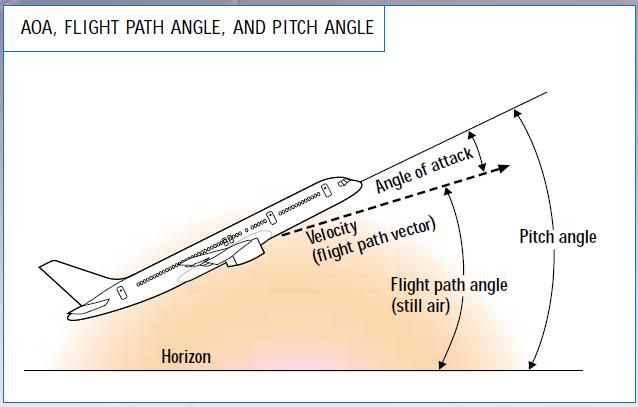
\includegraphics[width=0.75\textwidth]{Figures/flight_path_angle.png}
  \caption[Aircraft frames of reference]{$\gamma$ representation and frames of reference \cite{FPA}}
  \label{fig:flight_path_angle}
\end{figure}

After choosing the desired dynamics to control these variables, the equations above must be solved for both the thrust reference $T$, the desired AoA and $\psi$. From these last two, knowing the current roll angle $\theta$, the input for the fast dynamics controller is obtained. The desired dynamics were chosen as first order systems as
\begin{subequations}
\begin{equation}
\dot{V_a} = \dfrac{1}{\tau_{V_a}}(V_a^d-V_a)
\label{eq:va_dot_des}
\end{equation}
\begin{equation}
\dot{\gamma} = \dfrac{1}{\tau_{\gamma}}(\gamma^d-\gamma)
\label{eq:gamma_dot_des}
\end{equation}
\begin{equation}
\dot{\psi} = \dfrac{1}{\tau_{\psi}}(\psi^d-\psi)
\label{eq:psi_dot_des}
\end{equation}
\end{subequations}

The final step of the controller design will be to propose a guidance law to obtain the values of $V_a$, $\gamma$ and $\psi$ from the X,Y and Z reference values along time. For these laws was assumed that the position reference was given relative to a frame of reference with the origin on the surface, with the $Z$ axis pointing upwards. The guidance controller therefore implements the following equations, assuming the errors $\delta x = x_r - x$, $\delta y = y_r - y$ and $\delta z = z - z_r$.

\begin{subequations}
	\begin{gather}
	\delta V_a = \dfrac{1}{\tau_{V_a}}(\sqrt{\delta x^2 + \delta y^2 + \delta z^2})\\
	V_a^d= \delta V_a  + 100 ms^{-1}
	\end{gather}
	\begin{equation}
	\psi^d = atan2(\delta y,\delta x)
	\end{equation}
	\begin{equation}
	\gamma^d = \dfrac{1}{\tau_Z}\delta z
	\end{equation}
	\label{eq:guidance_law}
\end{subequations}
\section{Neural Network}
\label{section:NN}


Over the years, intelligent control techniques using neural networks have become a growing research topic, addressing the limitations of state-of-the-art model based controllers such as linear quadratic Gaussian, model predictive control, backstepping and gain scheduling \citep{SotA_IFCS}. Indeed, variation in the plat dynamics (e.g., due to payload changes, actuator or sensor degradation) deteriorate the performance and reference tracking error of the controller. To compensate for such errors, adaptive online neural networks have been studied and implemented in several works \cite{quad_NLI+NN}, \cite{NN_PID}, \cite{UAV_adaptive} and \cite{NN_NLI} to name a few. These however, have been applied almost exclusively to UAV aircrafts, especially multicopters. For this work a feedforward network with one hidden layer, one of the most widely implemented neural network architecture \cite{SotA_IFCS} was used.

\subsection{Network Architecture}
From an error-less nonlinear inversion, the pseuso-input $\tau$ would directly control $\ddot{\Omega}$ as seen previously. However, in case of inversion errors, that can be caused by several factors, the resulting in an equation similar to \ref{eq:system+error}, that $\tau = \ddot{\Omega}^d + \Delta$, where $\Delta = \ddot{\Omega}- \ddot{\Omega} ^d$. This method adds an adaptive component $\tau_{NN}$ to the pseudo input that will approximate the behaviour of the $\Delta$ error. The resulting control law will be given by $\tau + \tau_{NN} = \ddot{\Omega}^d + \Delta$, in which as $t \rightarrow \infty$, $\tau_{NN} \rightarrow \Delta$, thus adaptively minimizing inversion errors. To do so a simple neural network architecture was chosen: a network with a single hidden layer with therefore two sets of weights $V$ and $W$ that will need to be trained, corresponding to the input weights and the hidden layer ones. As for the activation functions for the hidden layer a sigmoid function was chosen, $sig(x)=\dfrac{1}{(1+e^{-x})}$. As the outputs must not be bound between $[0;1]$, the chosen output function was a linear one. Indeed sigmoid output functions are usually used in applications where the output must be a boolean value. A description of the chosen architecture can be found in figure \ref{fig:NN}. Different numbers of neurons were used and the results obtained will be discussed in chapter \ref{chapter:results}.

\begin{figure}[!htb]
  \centering
  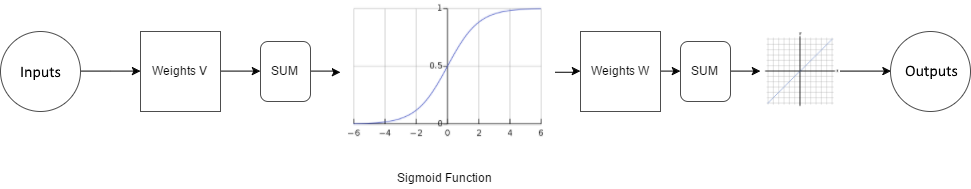
\includegraphics[width=1\textwidth]{Figures/NN.png}
  \caption[Neural Network diagram]{Neural Network diagram}
  \label{fig:NN}
\end{figure}

There are quite some challenges in designing a feed forward neural network. Besides choosing the number of layers and neurons per layer, the inputs of the network must also be chosen carefully. Some rules to choose the correct inputs are given in \cite{NN_inputs}:
\begin{itemize}
\item \textbf{Relevance}: Most important consideration to have while choosing inputs, this set must be sufficiently informative of the state of the system for the network to perform correctly. A NN will perform poorly is the output behaviour is not correlated to its input.
\item \textbf{Redundancy}: A large value of redundant and irrelevant input variables will not only increase the needed computational effort of the NN, but will also increase the difficulty to train the weights of the network and add noise to the system.
\end{itemize}

Another consideration about the chosen inputs that must also be taken into account is the range of values these might take. The sigmoid function $sing(x)$ used reaches around 75\% when $x=1$ and 100\% when $x=2$, as can be seen in figure \ref{fig:sigmoid}. For some cases the inputs might therefore need to be normalized. While this is quite a trivial task in the case of batch training, as the minimum and maximum value of each input is easily obtained before even starting training, such is not the case for online training, and a maximum and minimum value must be proposed \emph{a priori} for each input. The average of these values should also be close to zero. Should the input not be normalized and reach absolute values much greater than the unity, its activation function output would be constant and the system would therefore not react to input change. This, clearly, is not desirable. To map the input $x$ knowing its minimum and maximum values to its normalized equivalent $y$ the following equation is used

\begin{equation}
y=2\dfrac{x-x_{min}}{x_{max}-x_{min}}-1
\label{eq:normalisation}
\end{equation}

For this  particular case, the state variables of the fast dynamics where used as inputs of the network, namely $\Omega$ and $\dot{\Omega}$.

\begin{figure}[!htb]
  \centering
  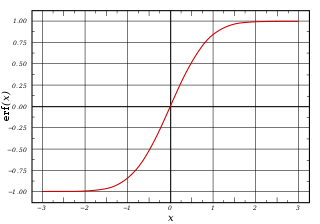
\includegraphics[width=0.5\textwidth]{Figures/sigmoid.png}
  \caption[Sigmoid Function]{Sigmoid Function}
  \label{fig:sigmoid}
\end{figure}

\subsection{Training Algorithm}

As mentioned in section \ref{section:background/NN}, a backpropagation algorithm was used to train both set of weights online. This algorithm, however, must have an error function that will be minimized by iteratively changing the values of the weights $V$ and $W$. As seen previously, due to inversion errors an error $\Delta$ will be present, where $\tau = \ddot{\Omega}^d + \Delta$. This error must be computed on each iteration to train the network to approximate this error. The error can be expressed as $\Delta=\tau - \ddot{\Omega}^d$. From the control law used to obtain $\tau$ (\ref{eq:linear_controller}) comes that
\begin{equation}
\Delta = -K_P(\Omega-\Omega^d)-K_D(\dot{\Omega}-\dot{\Omega}^d)
\label{eq:inversion_error}
\end{equation}
Finally the cost function used to train the network is given by

\begin{equation}
J=(\Delta-y_{NN})^2
\label{eq:NN_cost}
\end{equation}

The values of $\dot{V}$ and $\dot{W}$ must now be computing, using the gradient descent method described in section \ref{section:background/NN}. As the name suggest, the back propagation algorithm firstly computes the weight update values for the last layers, propagating the errors to update the previous weight set. The weights are constantly updated until the error's absolute value in lesser than a given value $\xi$, in which case these are kept constant as $\dot{V}=\dot{W}=0$. 
One of the parameters that must be tuned that has the largest impact on the performance of the network is the learning rate $\alpha$. This coefficient can also be thought of as the step size in incrementing the weight sets. Let $V^*$ and $W^*$ be the two ideal set of weights that, for a given input, result in an absolutely minimal cost function. A small value will allow the weights to converge to their ideal value, although taking many iterations to do so. A large learning rate however might converge faster, but might also overshoot and miss its optimal value. The results of the variation of this rate will be studied in chapter \ref{chapter:results}.

Finally, adding the online neural network to the baseline controller, the final control architecture is obtained. For the following chapter, the controller without the correction will be tested and compared in the same conditions to the same controller including the network. A simplified diagram of the controller can be seen in figure \ref{fig:full_controller}.
\begin{figure}[!htb]
  
  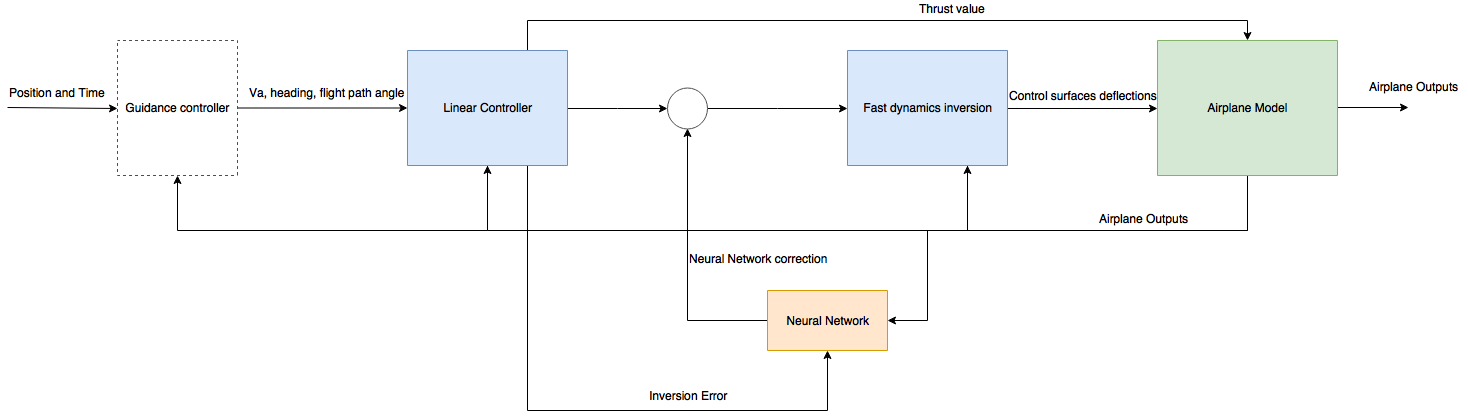
\includegraphics[width=1.1\textwidth]{Figures/full_controller.png}
  \caption[Diagram of the controller architecture]{Diagram of the controller architecture}
  \label{fig:full_controller}
\end{figure}
